\documentclass[12pt]{article}
\usepackage{gnuplottex}
\usepackage{csvsimple}
\usepackage{subcaption}
\usepackage{amsmath}
\usepackage{multirow}
\usepackage[top=4cm,bottom=4cm,left=4cm,right=4cm]{geometry}
\usepackage[justification=centering]{caption}
\usepackage[colorlinks,bookmarksopen,bookmarksnumbered,citecolor=green, linkcolor=red, urlcolor=green]{hyperref}



\title{Report of Deep Learning and Robotics}
\author{Xin Wu}

\begin{document}
\maketitle
\href{https://github.com/LinearAlgebraX/DeepLearningRobotic_cwk}{The github repo for this cwk}

\section{Literature review}
Deep learning models are of great significance in the field of robotics, allowing robots to learn complex operating tasks based on raw sensory data.\\

For the robot vision part, deep learning models, especially convolutional neural networks (CNN), are widely used in environment recognition as well as object detection, 
positioning and classification. SwipeBot\cite{SwipeBot} (Zherdev et al. 2023) is a recent typical example. It uses Deep CNN (ResNet-101 structure) to detect object classification and segmentation to distinguish movable and immovable objects and its estimated cost, 
which is used to calculate optimal path.\\

In SG-LSTM\cite{SG} (Bhaskara et al. 2023), the CNN-based group learning algorithm is also used to split the crowd into different "Groups". 
But also for this type of robot interaction task that requires processing sequence data and learning from sequence input\cite{review} (Lipton et al. 2015), 
long short-term memory (LSTM) - an improved recurrent neural network (RNN) is used . Represent each crowd/person as an LSTM for trajectory prediction\\

In addition, the generative adversarial network (GAN) in deep learning also has the potential to solve the challenge of low computational efficiency in finding 
valid robot configurations in high-dimensional robot systems when the configuration space is highly complex\cite{GAN} (Lembono et al. 2021)\\

Ideas and methods based on deep learning are undeniably profound for robotics and have excellent potential in sensing the environment and controlling them, 
but they also bring new problems. Reliance on data sets may potentially lead to performance degradation in unfamiliar environments, 
or even fatal risks due to data set poisoning\cite{BadNet} (Tianyu Gu et sl. 2019). The black-box nature of deep neural networks also makes the interpretability of learning strategies more complex, 
and its reliability and security are still a major challenge.

\section{Introduction}
Exploring the hyperparameter settings of a model for a specified data set has always been difficult to explain. This experiment aims to explore the method of finding the optimal solution for the hyperparameters of the image classification model, and gradually analyze the impact of each hyperparameter on the model performance. By systematically adjusting and evaluating the values of various hyperparameters, we aim to find the relatively optimal hyperparameter configuration to improve the performance and generalization ability of the image classification model.\\

In this report, the experimental design and the used data sets and neural network models will first be introduced. Subsequently, the adjustment results of hyperparameters will be described in detail and the impact of hyperparameters on model performance will be analyzed. Finally, the experimental results are summarized and the advantages and disadvantages of machine learning in the field of robotics are discussed.

\section{Experimental design}
Because of the black-box nature of the hidden layer of DNN, common methods of adjusting hyperparameters are often a posteriori. There are manual parameter adjustment, grid search, random search, Bayesian optimization, etc.
Considering the limitations of time cost and sample number, random search is first used to screen the hyperparameter group within a certain range and find a relatively optimal solution.\\
Then use the control variables to manually adjust parameters one by one to find the relationship between hyperparameters and model performance.\\

This experiment uses the common CIFAR10 as the target data set, and uses the ResNet\cite{ResNet} structure to avoid the degradation caused by too deep a network structure.\\


\section{Result}
In the random search stage, 30 training sessions of 10 epochs each were performed, and the accuracy returned by the validation set was used as the scoring criterion. As shown in Figure.1, the 28th hyperparameter configuration set has the highest accuracy and also has a low loss. is considered the closest to the optimal set of hyperparameters among these 30 searches.


\begin{figure*}[htbp]
    \centering
    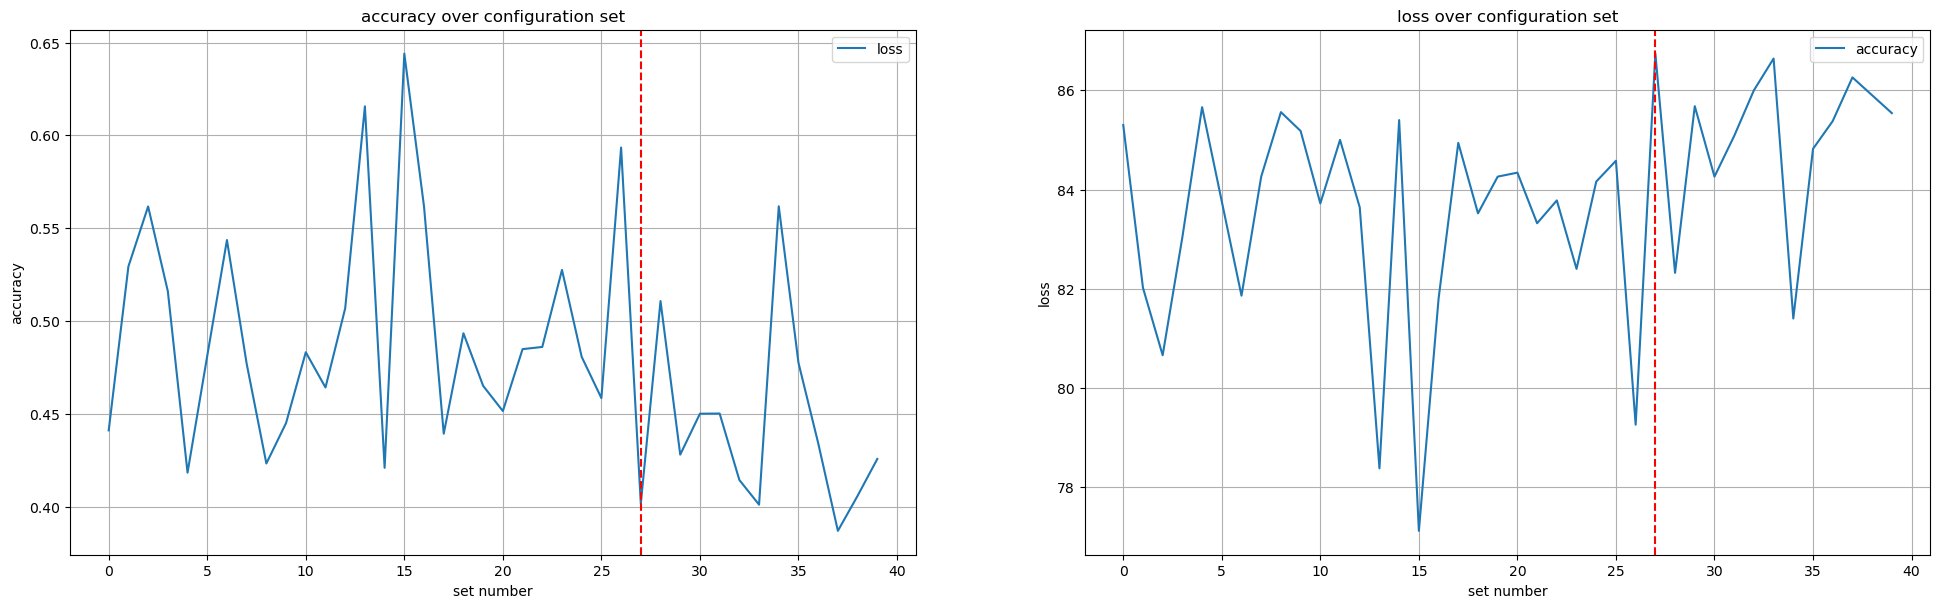
\includegraphics[width=\columnwidth,height=0.3\linewidth]{output.png}
    \caption{this is the result of random search, the red line is marked for the highest accuracy configuration}
\end{figure*}

In further manual parameter adjustment, when only a single hyperparameter is changed and the loss value during the training process is recorded, the trend shown in Figure.2 is obtained. We can see that for the learning rate, a higher learning rate means that the loss decreases faster, but it is not difficult to imagine that an excessively high learning rate may make it difficult for the model to converge.\\
As for the batch size, a larger batch size will make the model train faster, but from the image point of view, it does not give the model a higher upper limit. It can also be mentioned that when using a smaller batch size, the loss will fluctuate more drastically.


\begin{figure*}[htbp]
    \centering
    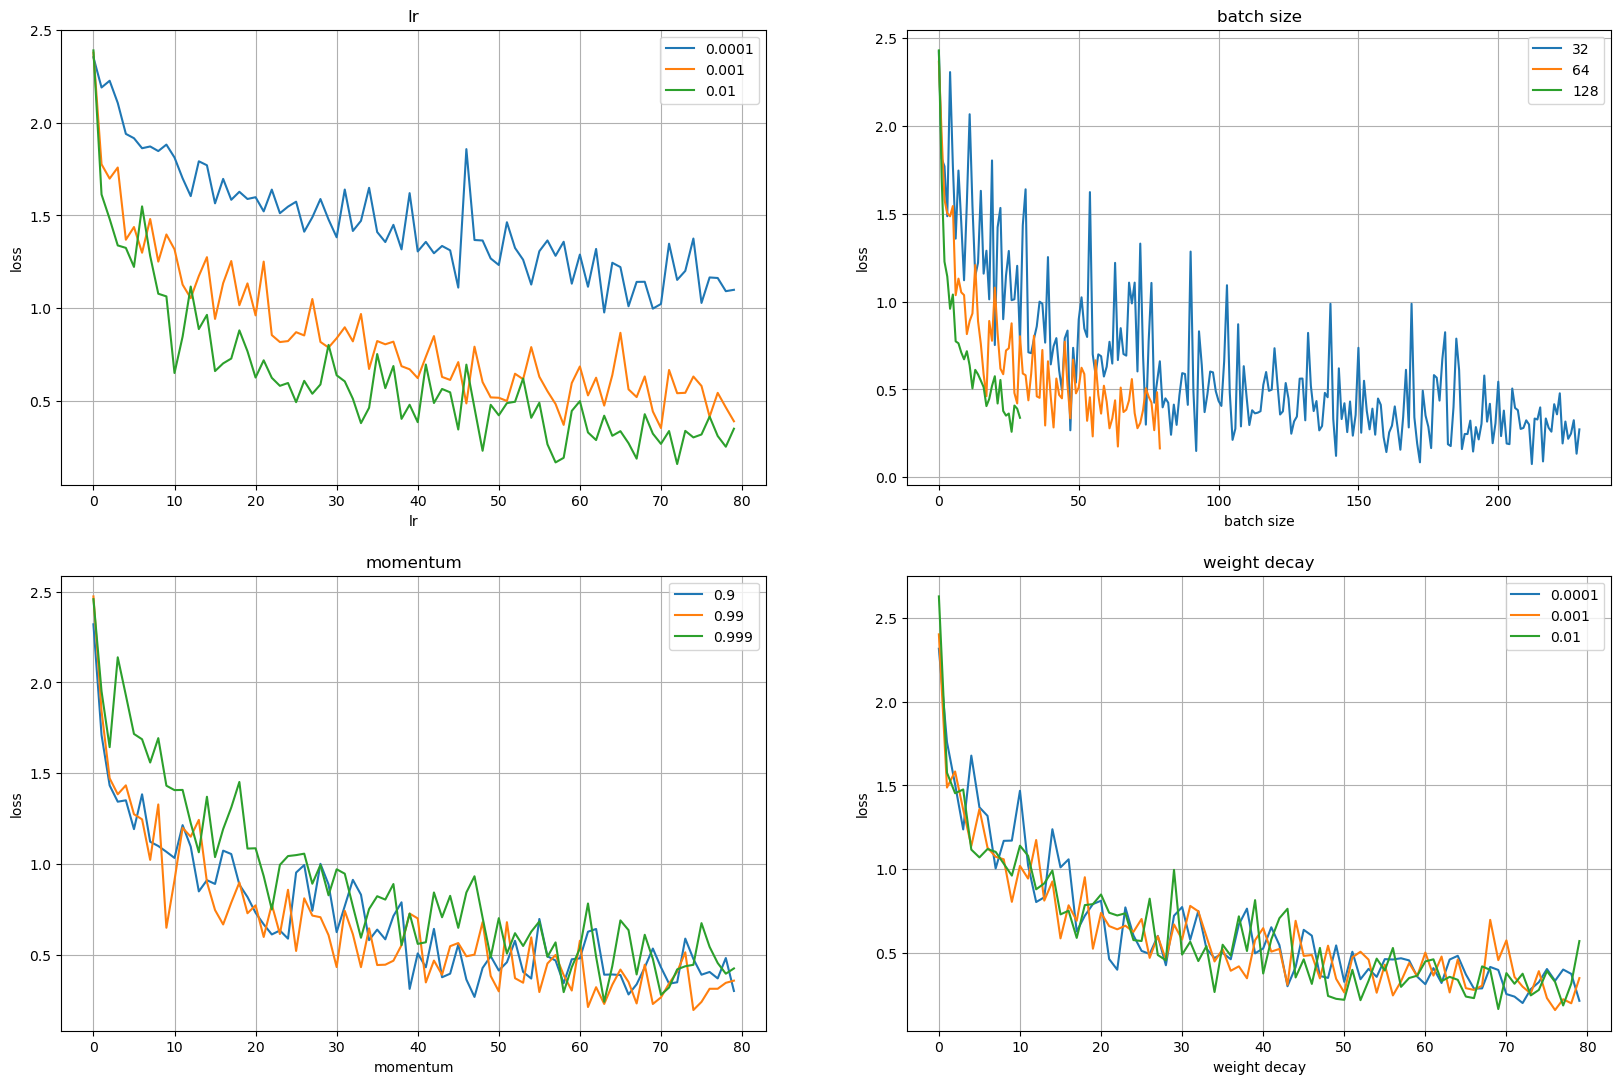
\includegraphics[width=\columnwidth,height=0.5\linewidth]{output2.png}
    \caption{this is the training loss recorded in control variable stage}
\end{figure*}

\section{Conclusion and Discussion of future simulation}
The following points can be summarized from this experiment: a higher learning rate will make the model learn faster, but it may make it difficult to converge. A larger batch size will allow the model to train faster and take up more memory. A smaller batch size will cause greater fluctuations in loss, but the overall impact cannot be seen. For different momentum and weight decay, there is no obvious difference in this experiment. \\
Overall, this simulation did not cover all hyperparameters. There are still many untested hyperparameters, such as epochs, different loss functions, optimizers and their tunable parameters.


\bibliographystyle{plain}
\bibliography{refPaper}
\end{document}